
\documentclass[aspectratio=169,14pt]{beamer}
\usetheme{default}\usecolortheme{default}\setbeamertemplate{navigation symbols}{}
\setbeamertemplate{footline}{\hfill{\scriptsize\color{covermuted}\insertframenumber/\inserttotalframenumber}\hspace{0.4cm}\vspace{0.15cm}}
\usepackage{fontspec}\usepackage{xeCJK}\setCJKmainfont{PingFang SC}[BoldFont=PingFang SC Semibold]\setmainfont{Helvetica Neue}[BoldFont=Helvetica Neue Bold]
\usepackage{xcolor}\usepackage{tikz}\usepackage{graphicx}\usepackage{fontawesome5}\usetikzlibrary{positioning,calc,arrows.meta,shadows}
\definecolor{bgmain}{RGB}{238,243,252}\definecolor{panel}{RGB}{238,244,255}\definecolor{factbg}{RGB}{246,242,235}\definecolor{coverprimary}{HTML}{2563EB}\definecolor{coveraccent}{HTML}{00A884}\definecolor{coverwarning}{HTML}{F59E0B}\definecolor{coverdark}{HTML}{1F2937}\definecolor{covermuted}{HTML}{64748B}\definecolor{titlecolor}{RGB}{30,30,30}\definecolor{muteddark}{RGB}{72,86,115}\definecolor{bluepanel}{RGB}{226,237,255}\definecolor{greenpanel}{RGB}{225,246,237}\definecolor{amberpanel}{RGB}{255,244,222}\definecolor{purplepanel}{RGB}{239,231,255}\setbeamercolor{background canvas}{bg=bgmain}
\newcommand{\plainbar}{\begin{tikzpicture}[remember picture, overlay]\fill[coverdark, opacity=0.07] (current page.south west) rectangle ([yshift=0.4cm]current page.south east);\draw[coveraccent, opacity=0.45, line width=0.8pt] ([yshift=0.4cm]current page.south west) -- ([yshift=0.4cm]current page.south east);\end{tikzpicture}}
\newcommand{\deckbackground}{\begin{tikzpicture}[remember picture, overlay]\fill[coverprimary!8] (current page.north west) rectangle (current page.south east);\fill[coverprimary!14] (current page.north west) ++(1.55,-1.35) circle (2.45cm);\fill[coveraccent!12] (current page.south east) ++(-1.9,1.45) circle (2.70cm);\fill[coverwarning!12] (current page.north east) ++(-2.9,-1.8) circle (0.85cm);\foreach \x in {-0.2,0.8,...,16.2} {\draw[coverprimary, opacity=0.045, line width=0.25pt] ([xshift=\x cm]current page.south west) -- ([xshift=\x cm]current page.north west);}\foreach \y in {-0.2,0.7,...,9.3} {\draw[coverprimary, opacity=0.04, line width=0.25pt] ([yshift=\y cm]current page.south west) -- ([yshift=\y cm]current page.south east);}\draw[coveraccent, opacity=0.38, line width=1.1pt] ([xshift=0.35cm,yshift=7.72cm]current page.south west) -- ++(3.25,0) -- ++(0.45,-0.45) -- ++(2.0,0);\draw[coverprimary, opacity=0.24, line width=1.0pt] ([xshift=9.35cm,yshift=8.25cm]current page.south west) -- ++(2.3,0) -- ++(0.55,-0.55) -- ++(3.2,0);\fill[coverdark, opacity=0.07] (current page.south west) rectangle ([yshift=0.42cm]current page.south east);\end{tikzpicture}}
\newcommand{\sectiontitle}[2]{\vspace{-0.52cm}\begin{center}{\fontsize{20}{24}\selectfont\bfseries\color{titlecolor} #1}\\[2pt]{\fontsize{9}{11}\selectfont\itshape\color{muteddark} #2}\end{center}\vspace{0.12cm}}
\newcommand{\portraitbox}[2]{\begin{tikzpicture}\node[draw=coverprimary!28, line width=0.7pt, fill=white, rounded corners=3pt, inner sep=2.5pt, drop shadow={shadow xshift=0.5pt, shadow yshift=-0.5pt, opacity=0.12}] {\includegraphics[width=2.4cm,height=2.9cm,keepaspectratio]{#1}};\end{tikzpicture}{\par\vspace{1pt}\fontsize{6.5}{7.5}\selectfont\color{covermuted} #2\par}}
\newcommand{\personslide}[9]{\begin{frame}\plainbar\vspace{-0.45cm}\begin{center}{\fontsize{22}{26}\selectfont\bfseries\color{coverdark} #1}\\[2pt]{\fontsize{9.5}{11.5}\selectfont\color{muteddark} #2}\end{center}\vspace{0.15cm}\begin{columns}[c]\begin{column}{0.22\textwidth}\centering #3\end{column}\begin{column}{0.28\textwidth}\begin{tikzpicture}\node[fill=greenpanel, rounded corners=4pt, inner xsep=6pt, inner ysep=5pt, text width=3.8cm, align=left] {{\fontsize{7}{8.5}\selectfont\bfseries\color{coveraccent!70!black} 获奖}\enspace{\fontsize{7}{8.5}\selectfont\color{coverdark!85} #4}\\[2.5pt]{\fontsize{7}{8.5}\selectfont\bfseries\color{coveraccent!70!black} 生卒}\enspace{\fontsize{7}{8.5}\selectfont\color{coverdark!85} #5}\\[2.5pt]{\fontsize{7}{8.5}\selectfont\bfseries\color{coveraccent!70!black} 身份}\enspace{\fontsize{7}{8.5}\selectfont\color{coverdark!85} #6}\\[2.5pt]{\fontsize{7}{8.5}\selectfont\bfseries\color{coveraccent!70!black} 机构}\enspace{\fontsize{7}{8.5}\selectfont\color{coverdark!85} #7}};\end{tikzpicture}\end{column}\begin{column}{0.48\textwidth}\begin{tikzpicture}\node[draw=coverprimary!35, fill=bluepanel, rounded corners=5pt, inner sep=7pt, text width=6.6cm, anchor=north west] at (0,0) {{\fontsize{8.6}{10.2}\selectfont\bfseries\color{coverprimary!82!black} 核心贡献}\\[3pt]{\fontsize{7.4}{9.2}\selectfont\color{coverdark!84} #8\\[3pt]\textbf{一句话：} #9}};\end{tikzpicture}\end{column}\end{columns}\end{frame}}

\begin{document}
\begin{frame}[plain]
\deckbackground
\begin{tikzpicture}[remember picture, overlay]
  \node[anchor=center, font=\fontsize{28}{34}\selectfont\bfseries, text=coverdark] at ([yshift=2.05cm]current page.center) {沃尔夫数学奖人物谱系};
  \node[anchor=center, font=\fontsize{15}{19}\selectfont, text=coverprimary!82!black] at ([yshift=0.86cm]current page.center) {第12集 \enspace·\enspace 泛函分析、算子理论与数理逻辑};
  \node[anchor=center, font=\fontsize{12}{16}\selectfont\bfseries, text=coveraccent!76!black] at ([yshift=0.10cm]current page.center) {Functional Analysis · Operator Theory · Logic};
  \draw[coveraccent, line width=1.4pt] ([yshift=-1.02cm, xshift=-4.55cm]current page.center) -- ([yshift=-1.02cm, xshift=4.55cm]current page.center);
  \node[anchor=center] at ([yshift=-1.90cm]current page.center) {\begin{tikzpicture}\node[rounded corners=8pt, fill=coverprimary!10, inner sep=4pt, minimum height=1.2em, font=\scriptsize\bfseries, text=coverprimary!85!black] at (-5.30,0) {Gelfand};\node[rounded corners=8pt, fill=coverprimary!10, inner sep=4pt, minimum height=1.2em, font=\scriptsize\bfseries, text=coverprimary!85!black] at (0.00,0) {Krein};\node[rounded corners=8pt, fill=coverprimary!10, inner sep=4pt, minimum height=1.2em, font=\scriptsize\bfseries, text=coverprimary!85!black] at (5.30,0) {Shelah};\end{tikzpicture}};
\end{tikzpicture}
\end{frame}
\begin{frame}
\plainbar
\sectiontitle{泛函分析、算子理论与数理逻辑}{Functional Analysis · Operator Theory · Logic}
\begin{center}\begin{tikzpicture}
  \node[draw=coverprimary!45, fill=bluepanel, rounded corners=5pt, inner sep=8pt, text width=11.2cm, align=left] at (0,1.05) {{\fontsize{8.3}{10}\selectfont\bfseries\color{coverprimary!80!black} 本集主线}\\[3pt]{\fontsize{7.4}{9.2}\selectfont\color{coverdark!84} 本集回到现代数学最抽象也最基础的层面：函数空间、线性算子、谱、表示论、模型论和集合论。沃尔夫奖在这里表彰的是改变语言本身的人。}};
  \node[draw=coverwarning!60, fill=amberpanel, rounded corners=5pt, inner sep=7pt, text width=11.2cm, align=center] at (0,-1.45) {{\fontsize{8.0}{9.8}\selectfont\bfseries\color{coverwarning!62!black} 开场问题}\\[-1pt]{\fontsize{7.4}{9}\selectfont\color{coverdark!82} 当对象太大、太抽象、甚至只是逻辑结构时，数学如何继续精确研究？}};
\end{tikzpicture}\end{center}
\end{frame}
\begin{frame}
\plainbar
\sectiontitle{人物路线图}{从早期奠基到现代前沿}
\begin{center}
\begin{tikzpicture}[milestone/.style={draw=coverprimary!45, fill=panel, rounded corners=4pt, inner xsep=4.0pt, inner ysep=5pt, align=center, font=\fontsize{5.9}{7.2}\selectfont\bfseries}, arrow/.style={-{Stealth}, draw=coveraccent, line width=0.7pt}]
\node[milestone, fill=bluepanel] (m0) at (-5.50,1.0) {1978\\Gelfand\\泛函};
\node[milestone, fill=greenpanel] (m1) at (0.00,1.0) {1982\\Krein\\算子};
\node[milestone, fill=amberpanel] (m2) at (5.50,1.0) {2001\\Shelah\\逻辑};
\draw[arrow] (m0) -- (m1);
\draw[arrow] (m1) -- (m2);
  \node[draw=coverprimary!38, fill=white, rounded corners=5pt, inner sep=7pt, text width=11.4cm, align=left] at (0,-1.25) {{\fontsize{8.0}{9.8}\selectfont\bfseries\color{coverprimary!80!black} 叙事线}\\[-1pt]{\fontsize{7.2}{8.8}\selectfont\color{coverdark!82} Gelfand 和 Krein 代表 20 世纪泛函分析与算子理论的高峰，Shelah 则把模型论和集合论推进到极深层次。本集作为系列收束，强调沃尔夫奖不仅奖励定理，也奖励重塑数学语言的人。}};
\end{tikzpicture}\end{center}
\end{frame}
\begin{frame}
\plainbar
\sectiontitle{本集的四个关键词}{观众需要记住的结构性线索}
\begin{columns}[T]
\begin{column}{0.49\textwidth}\begin{tikzpicture}
\node[draw=coverprimary!45, fill=bluepanel, rounded corners=5pt, inner sep=7pt, text width=6.0cm, anchor=north west] at (0,0) {{\fontsize{8.5}{10}\selectfont\bfseries\color{coverprimary!80!black} 1. 空间}\\[2pt]{\fontsize{7.3}{8.8}\selectfont\color{coverdark!82} 泛函分析把函数看成空间中的点，重写分析学语言。}};
\node[draw=coverprimary!45, fill=greenpanel, rounded corners=5pt, inner sep=7pt, text width=6.0cm, anchor=north west] at (0,-2.25) {{\fontsize{8.5}{10}\selectfont\bfseries\color{coveraccent!70!black} 2. 算子}\\[2pt]{\fontsize{7.3}{8.8}\selectfont\color{coverdark!82} 算子理论研究变换、谱和稳定性，连接分析与物理。}};
\end{tikzpicture}\end{column}
\begin{column}{0.49\textwidth}\begin{tikzpicture}
\node[draw=coverprimary!45, fill=amberpanel, rounded corners=5pt, inner sep=7pt, text width=6.0cm, anchor=north west] at (0,0) {{\fontsize{8.5}{10}\selectfont\bfseries\color{coverwarning!62!black} 3. 表示}\\[2pt]{\fontsize{7.3}{8.8}\selectfont\color{coverdark!82} 表示论用线性对象理解群和对称性。}};
\node[draw=coverprimary!45, fill=purplepanel, rounded corners=5pt, inner sep=7pt, text width=6.0cm, anchor=north west] at (0,-2.25) {{\fontsize{8.5}{10}\selectfont\bfseries\color{coverprimary!74!black} 4. 逻辑}\\[2pt]{\fontsize{7.3}{8.8}\selectfont\color{coverdark!82} 模型论和集合论研究数学结构的基础边界。}};
\end{tikzpicture}\end{column}
\end{columns}
\end{frame}
\personslide
  {Israel Gelfand}
  {以色列·盖尔范德：泛函分析与表示论的奠基者}
  {\portraitbox{images/Gelfand.jpg}{Photo: Wikipedia}}
  {1978（65岁）}
  {1913--2009}
  {苏联}
  {Moscow State University}
  {Gelfand 在泛函分析、群表示论、积分几何和广泛数学领域贡献巨大，是首届沃尔夫数学奖得主之一。}
  {他把抽象函数空间变成贯穿现代数学的基础语言。}
\personslide
  {Mark Krein}
  {马克·克雷因：算子理论、矩问题与逆散射}
  {\portraitbox{images/Krein.jpeg}{Photo: Wikipedia}}
  {1982（75岁）}
  {1907--1989}
  {苏联}
  {Odessa University}
  {Krein 在泛函分析、算子理论、矩问题和逆散射中贡献深远，长期因政治环境而未得到充分国际承认。}
  {他的工作体现了算子理论如何连接分析、谱和物理问题。}
\personslide
  {Saharon Shelah}
  {萨哈龙·谢拉：模型论与集合论的极高产大师}
  {\portraitbox{images/Shelah.jpg}{Photo: Wikipedia}}
  {2001（56岁）}
  {1945--}
  {以色列}
  {Hebrew University of Jerusalem}
  {Shelah 在数理逻辑、模型论和集合论中贡献巨大，以极高产和深刻技术著称，改变了稳定性理论等方向。}
  {他展示了逻辑不是数学外壳，而是数学结构本身的研究对象。}
\begin{frame}
\plainbar
\sectiontitle{第12集的主线}{泛函分析、算子理论与数理逻辑}
\begin{center}\begin{tikzpicture}[block/.style={draw=coverprimary!42, fill=white, rounded corners=5pt, inner sep=6pt, text width=3.0cm, align=center, font=\fontsize{7.0}{8.5}\selectfont}, arrow/.style={->, draw=coveraccent, line width=0.85pt}]
  \node[block, fill=bluepanel] (a) at (-4.9,1.25) {\textbf{起点}\\基础语言}; \node[block, fill=greenpanel] (b) at (-1.65,1.25) {\textbf{工具}\\结构方法}; \node[block, fill=amberpanel] (c) at (1.65,1.25) {\textbf{突破}\\核心定理}; \node[block, fill=purplepanel] (d) at (4.9,1.25) {\textbf{影响}\\跨域应用};
  \draw[arrow] (a) -- (b); \draw[arrow] (b) -- (c); \draw[arrow] (c) -- (d);
  \node[draw=coverwarning!65, fill=factbg, rounded corners=5pt, inner sep=7pt, text width=11.1cm, align=left] at (0,-1.35) {{\fontsize{8.0}{9.8}\selectfont\bfseries\color{coverwarning!62!black} 一句话总结}\\[-1pt]{\fontsize{7.4}{9}\selectfont\color{coverdark!84} Gelfand 和 Krein 代表 20 世纪泛函分析与算子理论的高峰，Shelah 则把模型论和集合论推进到极深层次。本集作为系列收束，强调沃尔夫奖不仅奖励定理，也奖励重塑数学语言的人。}};
\end{tikzpicture}\end{center}
\end{frame}
\begin{frame}
\plainbar
\sectiontitle{下一步}{专题系列衔接}
\begin{center}\begin{tikzpicture}
  \node[draw=coverwarning!60, fill=coverwarning!12, rounded corners=5pt, inner sep=7pt, text width=10.5cm, align=center] at (0,1.4) {{\fontsize{8.4}{10}\selectfont\bfseries\color{coverwarning!65!black} 系列收束}\\[-1pt]{\fontsize{7.4}{9}\selectfont\color{coverdark!80} 从奖项看 20 世纪数学主干：语言、结构、空间、随机、计算与逻辑。}};
  \node[draw=coverprimary!45, fill=bluepanel, rounded corners=5pt, inner sep=8pt, text width=10.5cm, align=center] at (0,-1.35) {{\fontsize{10.5}{12.8}\selectfont\bfseries\color{coverprimary!82!black} 沃尔夫数学奖人物谱系：12 集主题地图}};
\end{tikzpicture}\end{center}
\end{frame}
\end{document}
